\documentclass[convert = false, tikz]{standalone}
\usepackage[utf8]{inputenc}
\usepackage{tikz}
\usetikzlibrary{automata, positioning, arrows}

\usepackage{../../../../style_automata}

% arara: pdflatex
% arara: latexmk: { clean: partial }
\begin{document}
    \tikzset{
    node distance=2.5cm, % specifies the minimum distance between two nodes.
    }
    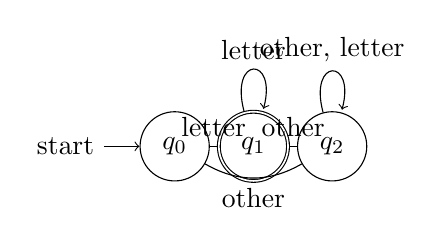
\begin{tikzpicture}
        \node[state, initial] (q0) {$q_0$};
        \node[state, accepting, right of=q0] (q1) {$q_1$};
        \node[state, right of=q1] (q2) {$q_2$};
        \draw (q1) edge[loop above] node{letter} (q1)
        (q2) edge[loop above] node{other, letter} (q2)
        (q0) edge[above] node{letter} (q1)
        (q1) edge[above] node{other} (q2)
        (q0) edge[bend right, below] node{other} (q2);
    \end{tikzpicture}
\end{document}